\subsection{Observables} \label{sec:WBoson_Results_Observables}

%%------------------------------------------------------------%%
\subsubsection{W boson cross sections} \label{sec:WBoson_Results_Observables_CrossSection}

The differential \WToMuNu cross sections are calculated by dividing the efficiency-corrected \WToMuNu yields ($N_{corr}$) over the recorded integrated luminosity (\Lumi) times the bin width ($\Delta\eta_{CM}$), as described below: 

\begin{equation}
\frac{d\sigma^{\pm}}{d\eta_{CM}}(\eta_{CM}) = \frac{N^{\pm}_{corr}(\eta_{CM})}{\Delta\eta_{CM}\Lumi}
\label{eq:CrossSection}
\end{equation}

The results of the production cross sections for \WToMuNuPl and \WToMuNuMi, as a function muon \etaCM, are shown in \fig{fig:CrossSection_WToMu_PA}. The vertical error bars represent the statistical uncertainties from the measured \WToMuNu yields, while the brackets show the statistical and total systematic uncertainties summed in quadrature. The global integrated luminosity uncertainty of $\pm$3.4\%~\cite{LUMI} is not shown.

\begin{figure}[htbp]
 \begin{center}
  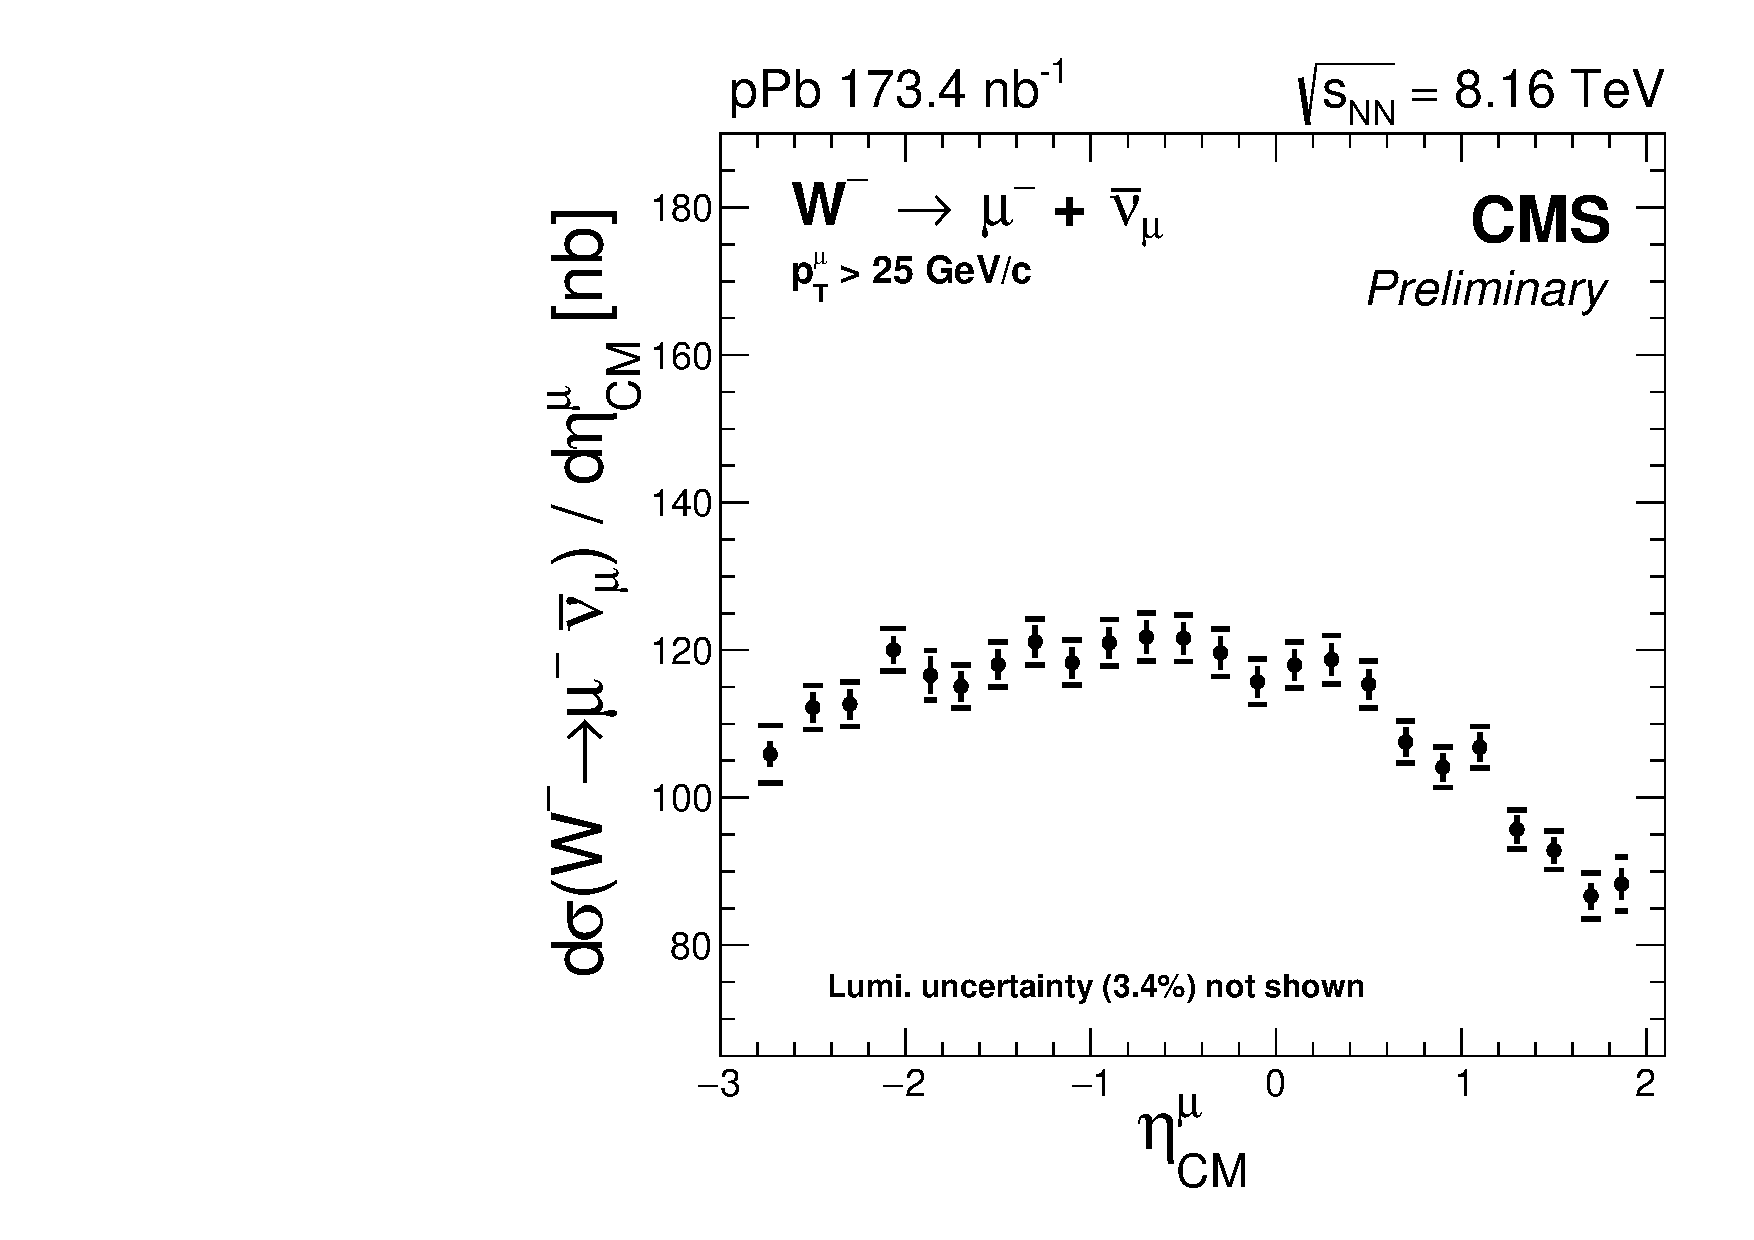
\includegraphics[width=0.45\textwidth]{Figures/WBoson/Results/DATA/PA/Cross_Section/gr_WToMuMi_PA_Cross_Section_EffTnP_Nominal.pdf}
%%
  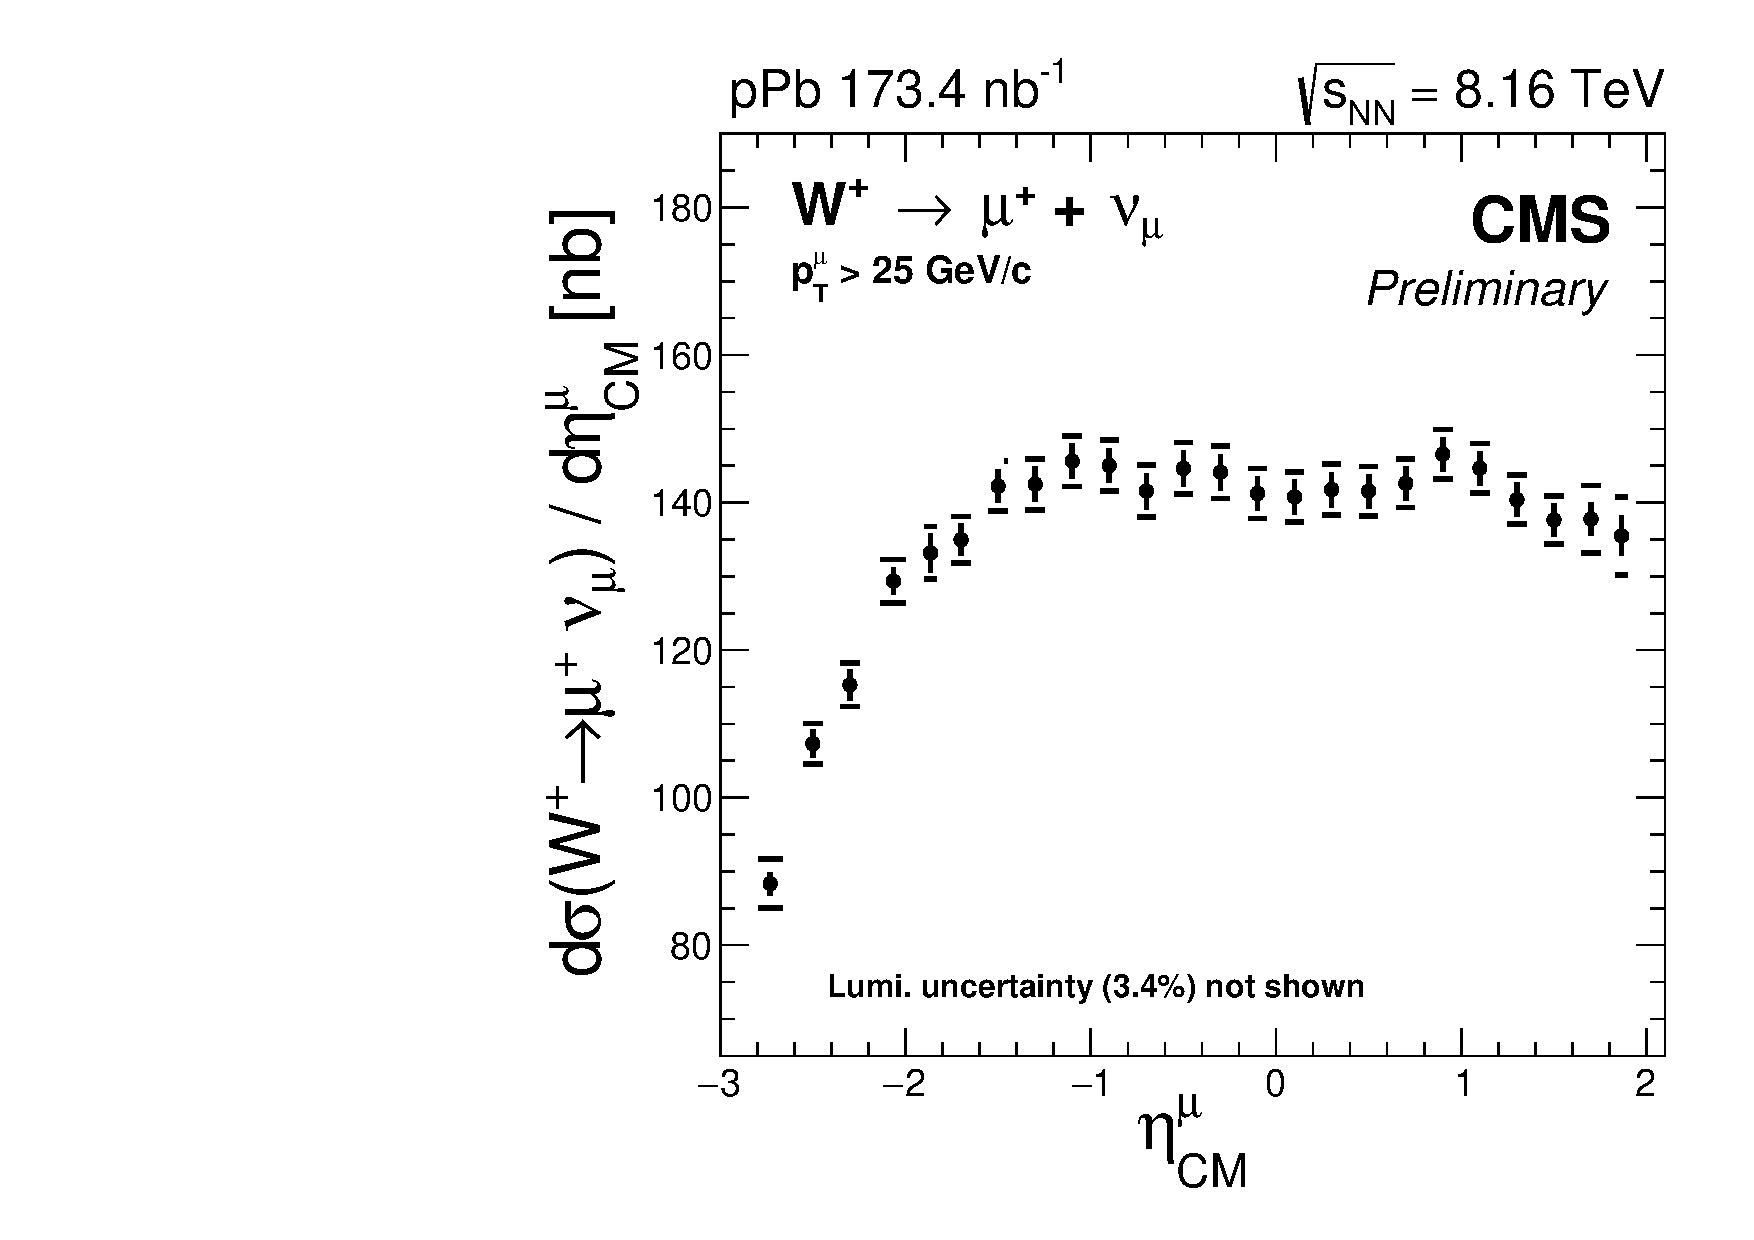
\includegraphics[width=0.45\textwidth]{Figures/WBoson/Results/DATA/PA/Cross_Section/gr_WToMuPl_PA_Cross_Section_EffTnP_Nominal.pdf}
 \end{center}
 \caption{Production cross sections for \WToMuNuPl (left) and \WToMuNuMi (right), as a function of the muon pseudorapidity in the center-of-mass frame. The brackets represent the statistical and systematic uncertainties summed in quadrature, while the error bars show the statistical uncertainties only. The global luminosity uncertainty of $\pm$3.4\%~\cite{LUMI} is not shown. }
 \label{fig:CrossSection_WToMu_PA}
\end{figure}

The opposite trend seen between the {\PWp} and {\PWm} boson differential cross sections is expected from parity violation of the electroweak interaction. The {\PWp} bosons decay to a right-handed antimuon boosted in the opposite direction, while the {\PWm} bosons decay to a left-handed muon along the direction of the {\PWm} boson. As a consequence, the {\PGmp} and {\PGmm} yields differ as a function of the muon \etaCM.

%%------------------------------------------------------------%%
\subsubsection{Muon charge asymmetry} \label{sec:WBoson_Results_Observables_ChargeAsymmetry}

The muon charge asymmetry ($C_{\mu}$) between \WToMuNuMi and \WToMuNuPl processes and its corresponding uncertainty are defined in \eq{eq:MuonChargeAsymmetry} and \eq{eq:MuonChargeAsymmetryStatError}, respectively.

\begin{equation}
C_{\mu}(\etaCM) = \frac{ N^{+}_{corr}(\etaCM) - N^{-}_{corr}(\etaCM) }{ N^{+}_{corr}(\etaCM) + N^{-}_{corr}(\etaCM) }
\label{eq:MuonChargeAsymmetry}
\end{equation}

\begin{equation}
\delta{C_{\mu}(\etaCM)} = 
\left(\frac{2 \times N^{+}_{corr}(\etaCM) \times N^{-}_{corr}(\etaCM)}{\left(N^{+}_{corr}(\etaCM)+N^{-}_{corr}(\etaCM)\right)^{2}}\right) \times
\sqrt{ 
	\left(\frac{\delta{N^{+}_{corr}(\etaCM)}}{N^{+}_{corr}(\etaCM)}\right)^{2} +
	\left(\frac{\delta{N^{-}_{corr}(\etaCM)}}{N^{-}_{corr}(\etaCM)}\right)^{2}
}
\label{eq:MuonChargeAsymmetryStatError}
\end{equation}

The uncertainties correlated in muon charge, such as the integrated luminosity uncertainty of 3.4$\%$ and the systematic components of the tag-and-probe correction uncertainties (<2.8$\%$), cancel in the measurement of the muon charge asymmetry. The measured muon charge asymmetry is shown in \fig{fig:ChargeAsymmetry_WToMu_PA} as a function muon $\eta_{CM}$.

\begin{figure}[htbp]
 \begin{center}
  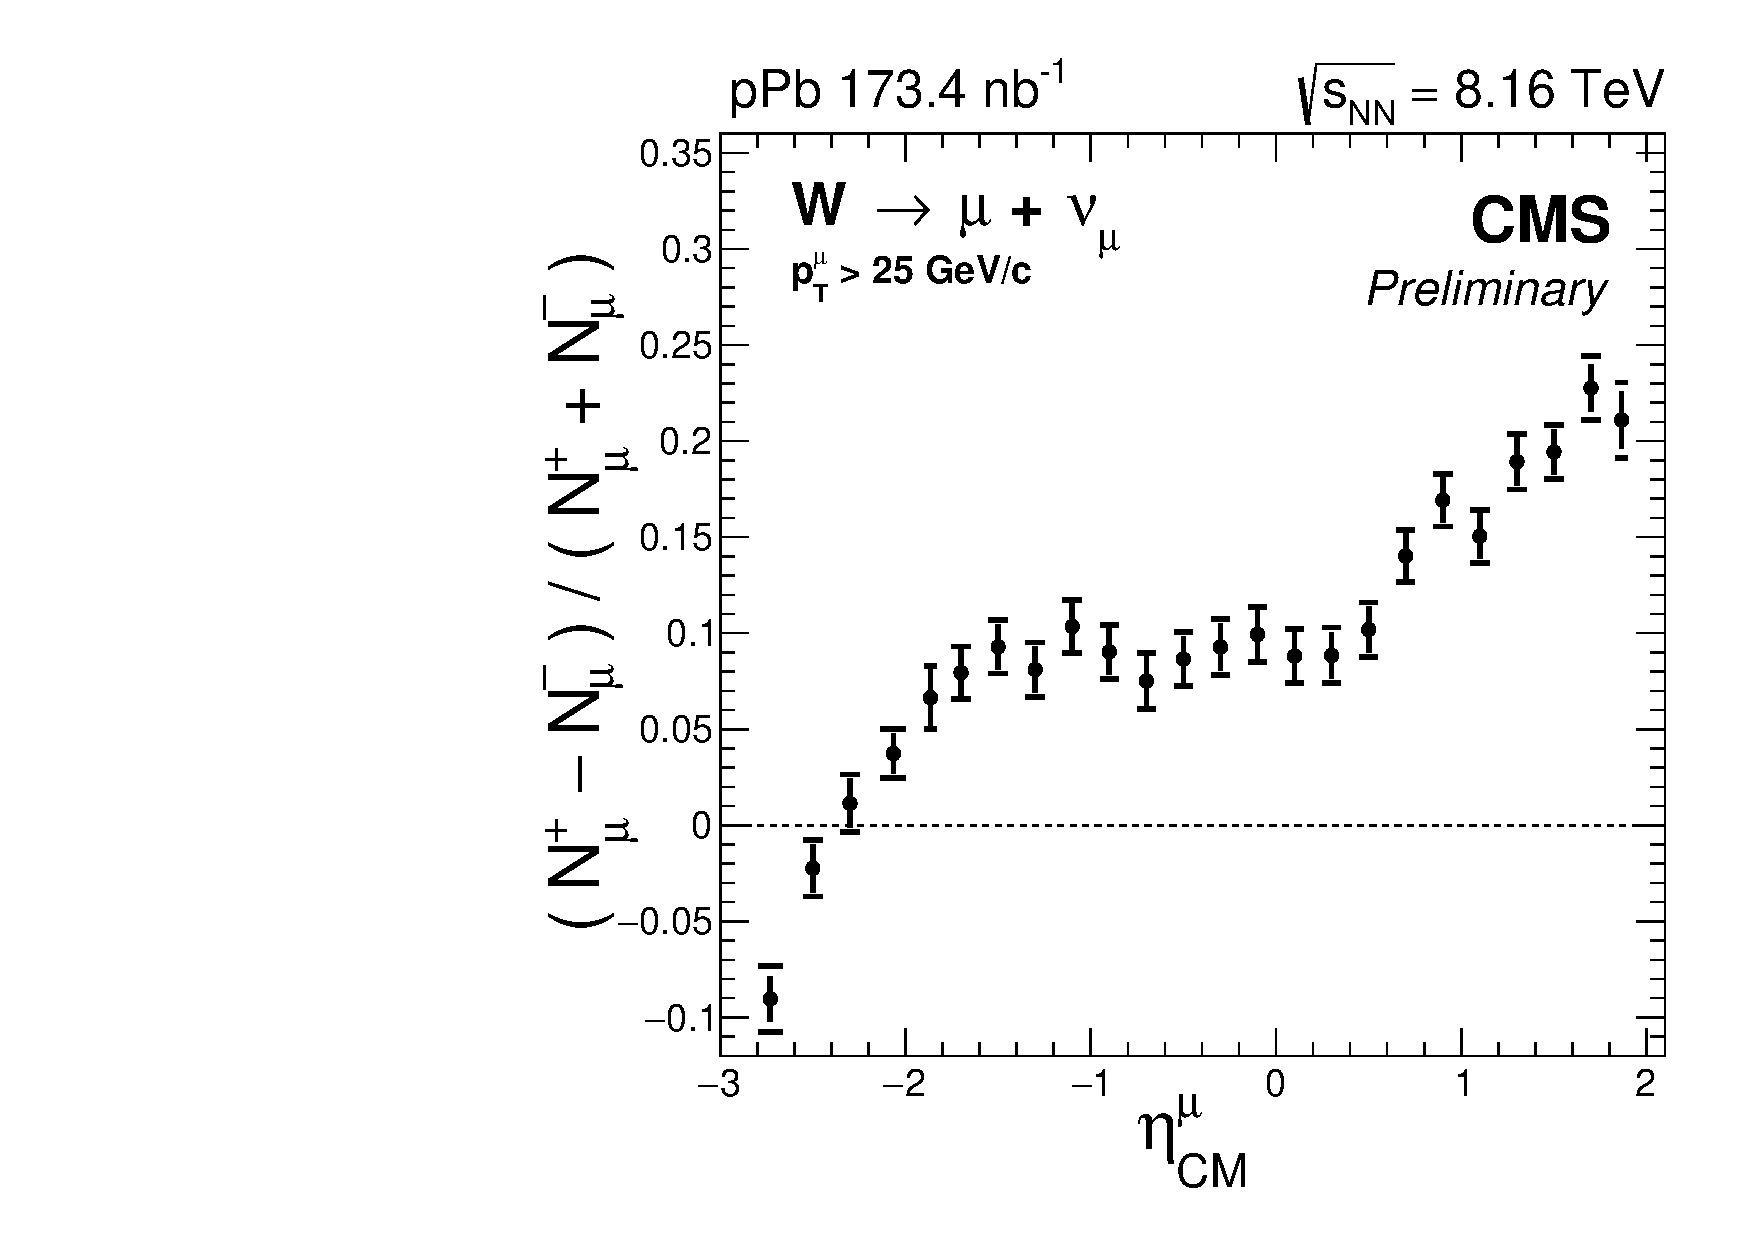
\includegraphics[width=0.45\textwidth]{Figures/WBoson/Results/DATA/PA/Charge_Asymmetry/gr_WToMuInc_PA_Charge_Asymmetry_EffTnP_Nominal.pdf}
 \end{center}
 \caption{Muon charge asymmetry as a function of the muon pseudorapidity in the center-of-mass frame. The brackets represent the statistical and systematic uncertainties summed in quadrature, while the error bars show the statistical uncertainties only.}
 \label{fig:ChargeAsymmetry_WToMu_PA}
\end{figure}

%%------------------------------------------------------------%%
\subsubsection{Muon forward-backward ratios} \label{sec:WBoson_Results_Observables_ForwardBackwardRatio}

The muon forward-backward ratio ($R_{FB}$) is defined as the ratio of the \WToMuNu yields extracted in the forward \etaCM bin divided by its backward counterpart. By convention, the forward region corresponds to the proton-going direction while the backward region corresponds to the Pb-going direction. The muon forward-backward ratio is measured for each muon charge separately, and also considering all muons. The $R_{FB}$ is defined in \eq{eq:MuonForwardBackwardAsymmetry} and its uncertainty is computed using \eq{eq:MuonForwardBackwardAsymmetryStatError}.

\begin{equation}
R_{FB}(\eta) = \frac{ N_{corr}(+\eta_{CM}) }{ N_{corr}(-\eta_{CM}) }
\label{eq:MuonForwardBackwardAsymmetry}
\end{equation}

\begin{equation}
\delta{R_{FB}(\eta_{CM})} = R_{FB}(\eta_{CM}) \times \sqrt{
	\left(\frac{\delta{N_{corr}(+\eta_{CM})}}{N_{corr}(+\eta_{CM})}\right)^{2} +
	\left(\frac{\delta{N_{corr}(-\eta_{CM})}}{N_{corr}(-\eta_{CM})}\right)^{2}
}
\label{eq:MuonForwardBackwardAsymmetryStatError}
\end{equation}

The results of the forward-backward ratio of all muons and the ratio for \WToMuNuMi and \WToMuNuPl decays, are shown in \fig{fig:ForwardBackwardRatio_WToMu_PA}. The uncertainties correlated in muon pseudorapidity, such as the integrated luminosity uncertainty of 3.4$\%$, the event activity reweighing uncertainty and the systematic uncertainties due to the electroweak backgrounds, are strongly reduced.

\begin{figure}[htbp]
 \begin{center}
  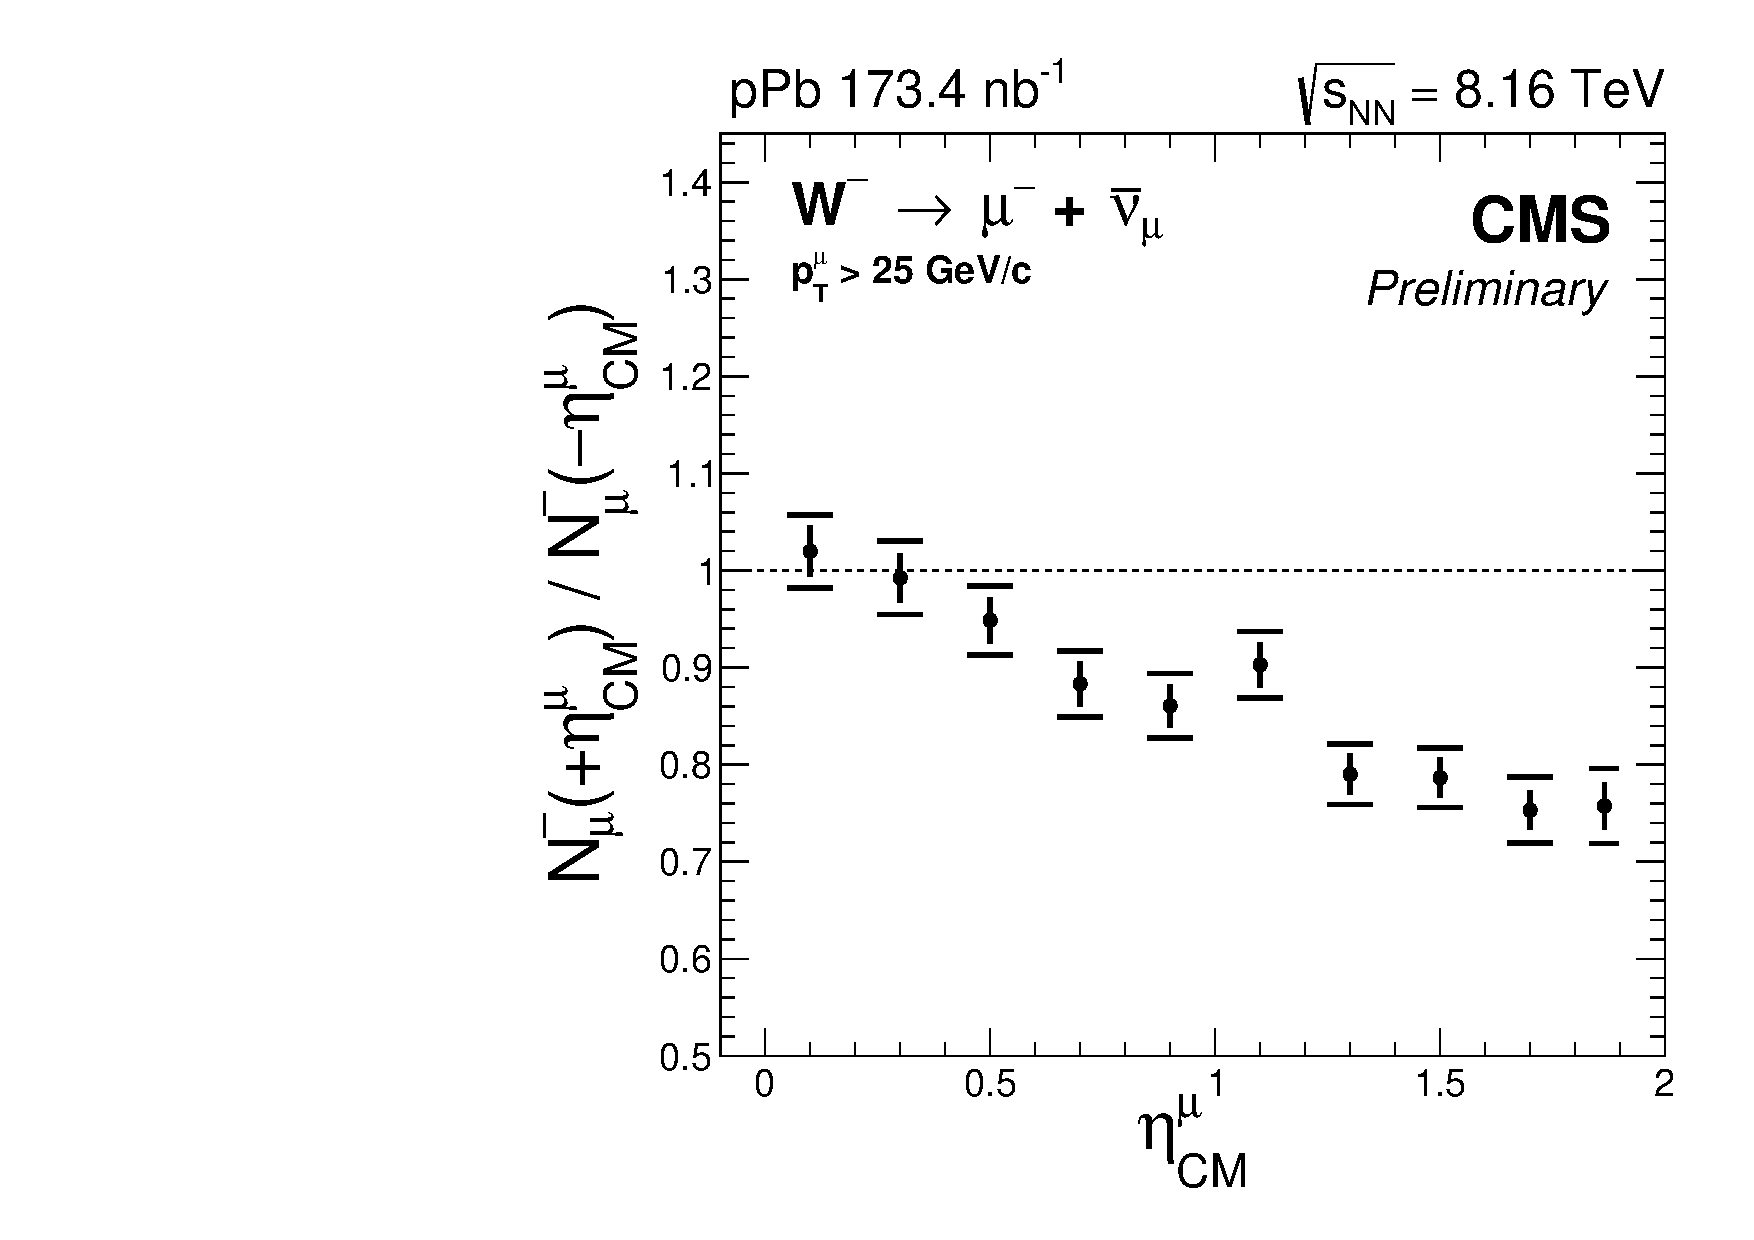
\includegraphics[width=0.32\textwidth]{Figures/WBoson/Results/DATA/PA/ForwardBackward_Ratio/gr_WToMuMi_PA_ForwardBackward_Ratio_EffTnP_Nominal}
%%
  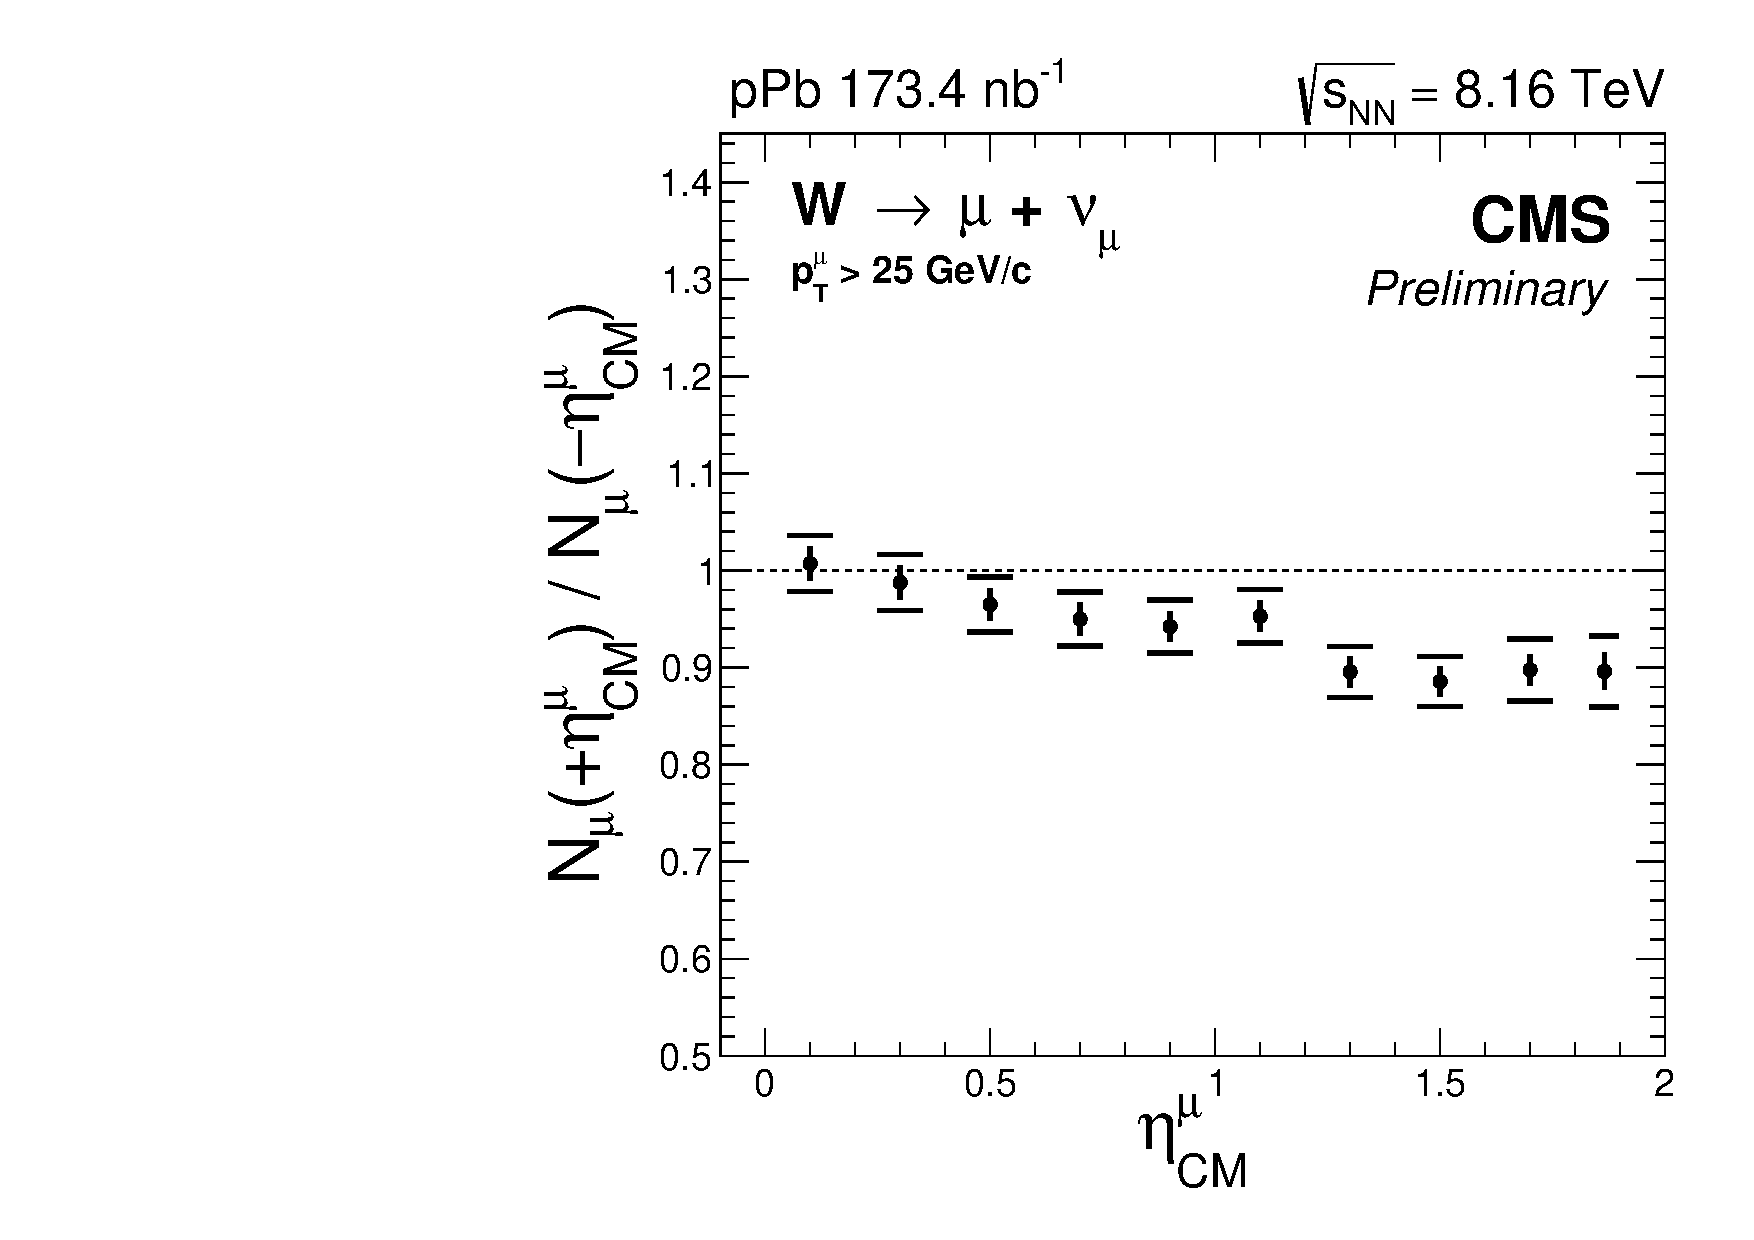
\includegraphics[width=0.32\textwidth]{Figures/WBoson/Results/DATA/PA/ForwardBackward_Ratio/gr_WToMuInc_PA_ForwardBackward_Ratio_EffTnP_Nominal}
%%
  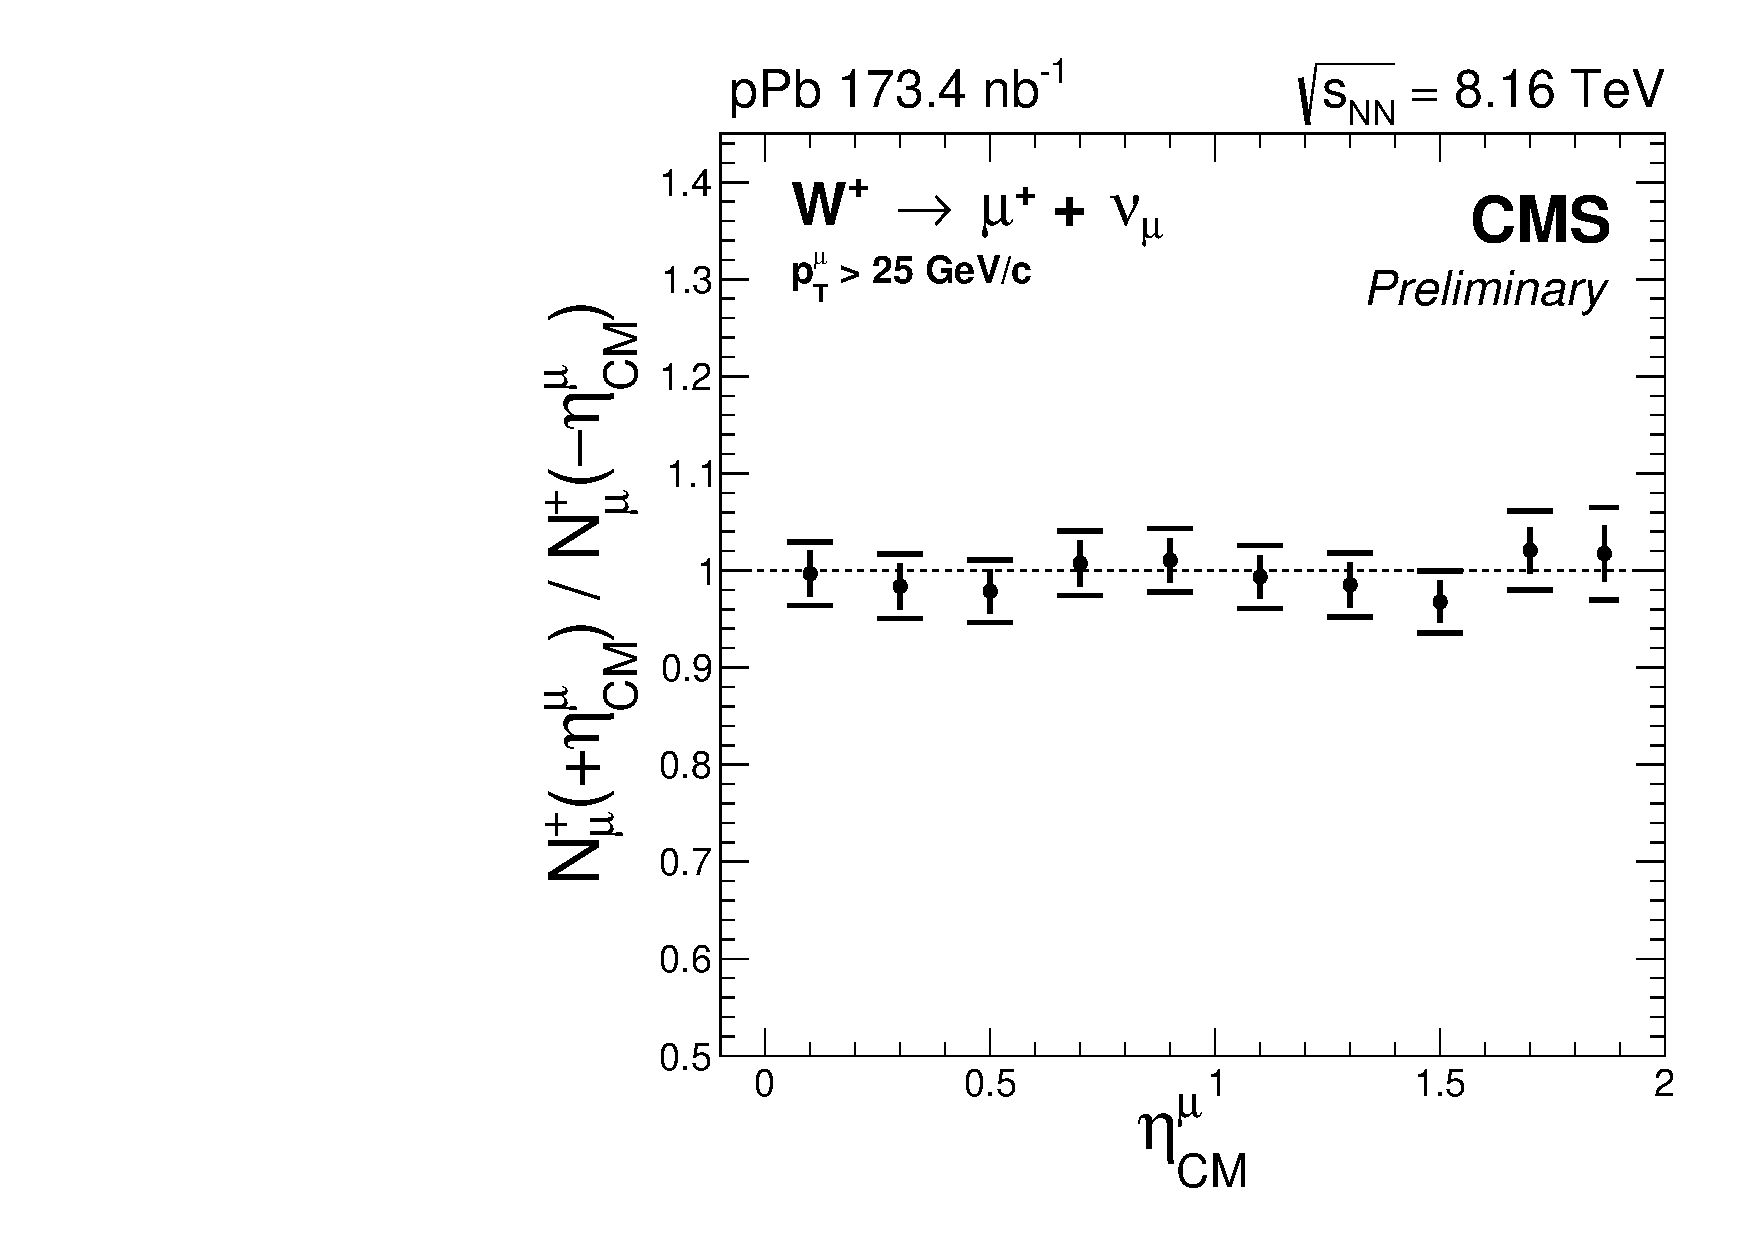
\includegraphics[width=0.32\textwidth]{Figures/WBoson/Results/DATA/PA/ForwardBackward_Ratio/gr_WToMuPl_PA_ForwardBackward_Ratio_EffTnP_Nominal}
 \end{center}
 \caption{Forward-backward ratios, for the positive (left), all (middle) and negative (right) charged muons. The brackets represent the statistical and systematic uncertainties summed in quadrature, while the error bars show the statistical uncertainties only.}
 \label{fig:ForwardBackwardRatio_WToMu_PA}
\end{figure}


% END OF SUBSECTION
